% Consolidated report.tex for the Banking Management System.
\documentclass[12pt,a4paper]{report}
\usepackage[margin=1in]{geometry}
\usepackage{graphicx}
\usepackage{float}
\usepackage{hyperref}
\usepackage{natbib}
\usepackage{verbatim}
\usepackage{tabularx}






\graphicspath{{figures/}}
\setlength{\parindent}{0pt}
\setlength{\parskip}{0.6em}




% ------- Project metadata -------
\title{Banking Management System}
\date{27 July 2026}
\newcommand{\coursecode}{COMP XXXX}
\newcommand{\yeargroup}{I}
\newcommand{\semester}{II}
\newcommand{\groupname}{Computer Science}
\newcommand{\memberA}{Trilochan Sharma}
\newcommand{\memberB}{Ujjwal Upadhya}
\newcommand{\memberC}{Adarsha Shah}
\newcommand{\memberD}{Saurav Shah}
\newcommand{\supervisorname}{Aayush Paudel}

\begin{document}

\begin{titlepage}
  \centering
  \vspace*{1cm}
  \includegraphics[width=4cm]{logo-200.png}\\[0.8cm]
  {\LARGE Kathmandu University}\\[0.3cm]
  {\large Department of Computer Science and Engineering}\\[1.2cm]
  {\Huge\bfseries Banking Management System}\\[0.8cm]
  {\large (For partial fulfillment of 1st Year / 2nd Semester)}\\[1.2cm]
  {\Large Submitted by:}\\[0.4cm]
  {\memberA \\ \memberB \\ \memberC \\ \memberD}\\[1cm]
  {\large Submitted to: \\ \supervisorname \\ Department of Computer Science and Engineering}\\[1cm]
  {27 July 2026}
\end{titlepage}

\cleardoublepage
\section*{Acknowledgements}
\addcontentsline{toc}{section}{Acknowledgements}
We would like to express our sincere gratitude to our supervisor, faculty members, and the Department of Computer Science and Engineering at Kathmandu University for their guidance and support throughout this project.

\cleardoublepage
\section*{Abstract}
\addcontentsline{toc}{section}{Abstract}
This report presents the design and implementation of a Banking Management System developed as a semester project. The system is a console-based C++ application backed by SQLite and supports user registration, authentication, account balance tracking, fund transfer requests, and admin approval workflows. The project was implemented using modular C++ design principles, parameterized SQL operations, and a persistent local database so that core banking functions can be demonstrated reliably in an academic setting.

The implementation emphasizes secure account handling, transaction traceability, and maintainability. It demonstrates how a lightweight database-driven application can model essential banking operations such as account creation, balance management, transfer processing, and admin oversight. The project was built using CMake and tested on a Windows environment with the MinGW toolchain.

\noindent\textbf{Keywords:} Banking System, C++, SQLite, Database Management, Console Application, Transaction Approval

\cleardoublepage
\tableofcontents
\listoffigures
\listoftables

\cleardoublepage
\pagenumbering{arabic}

\chapter{Introduction}
Banking systems are essential software applications that help manage customer accounts, funds, and transaction records in a secure and organized manner. This project was developed to demonstrate how a small-scale, database-driven banking system can be built using the C++ programming language and SQLite. The system supports two main user roles: customers and administrators.

\section{Problem Statement}
A basic banking system should provide secure account access, accurate balance maintenance, and a controlled transfer process. In many student-level implementations, these requirements are simplified to focus on the core database and application logic. This project addresses that need by implementing a console-based banking application with user authentication, account creation, transfer requests, and admin approval.

\section{Objectives}
The main objectives of the project were to:
\begin{itemize}
  \item implement a secure user registration and login system;
  \item create per-user bank accounts with balance tracking;
  \item enable fund transfer requests that require admin approval;
  \item design a simple but reliable database schema for users, accounts, and transactions; and
  \item present the system clearly through documentation and a sample run transcript.
\end{itemize}

\section{Scope of the Project}
The scope of this project includes basic customer and administrator functionality, local storage using SQLite, and a console-based interactive interface. It does not aim to replace full-scale banking software, but rather to provide a practical academic implementation of essential banking operations.

\section{Report Organization}
This report is organized into five chapters. Chapter 1 introduces the project goals, scope, and core objectives. Chapter 2 reviews related academic work and common design patterns for banking applications. Chapter 3 describes the system architecture, data model, and implementation methodology. Chapter 4 explains the actual implementation, testing, and results. Chapter 5 concludes with the project outcomes and suggestions for future work.

\chapter{Literature Review and Related Work}
Academic banking management systems are typically designed around secure login, account handling, transaction recording, and administrative oversight. Many student projects use lightweight database-backed console applications to demonstrate these concepts while keeping the implementation manageable.

This work follows the standard academic patterns of:
\begin{itemize}
  \item modular separation between interface, business logic, and persistence,
  \item use of a relational database for reliable data storage,
  \item transaction approval workflows to model basic banking checks and balances,
  \item clear documentation of system design and expected behavior.
\end{itemize}

The implementation here is intentionally lightweight compared to production banking systems, prioritizing clarity and correctness over advanced features such as distributed transaction processing, encrypted communication, or real-time concurrency control.

\chapter{System Design and Methodology}
\section{System Overview}
The Banking Management System is organized into three main layers: the user interface layer, the application logic layer, and the database layer. The user interface provides console menus for customers and administrators. The application logic handles authentication, account management, transfer submission, and approval processing. The database layer stores persistent data such as user credentials, account balances, transaction histories, and request statuses.

\subsection{Architectural Design}
The architecture emphasizes separation of concerns so that each part of the system does one thing well. The presentation layer is responsible for interaction with the user and menu navigation. The application layer contains the business rules and validation logic. The persistence layer encapsulates all SQL access and database state.

\subsection{Design Rationale}
This design aids maintainability and makes it easier to extend the system. By separating concerns, the project can add new features later without deeply changing other components. It also allows test scenarios to focus on specific functionality such as authentication, account updates, or transaction approval.

\section{Database Design}
The database schema includes tables for users, accounts, and transactions. Each transaction record stores the sender account, recipient account, amount, timestamp, and pending or approved status.

The system uses parameterized SQL statements to prevent SQL injection and to ensure safe, consistent database updates. The database design supports both customer-facing account operations and administrator approval flows.

\section{Implementation Approach}
The implementation was carried out in a modular style. Core components include authentication, account management, transfer processing, and approval handling. Each component is implemented in its own source file and interacts through well-defined interfaces.

The project was built using CMake and tested as a standalone executable on Windows. The development approach was iterative: first the database schema and basic data access, then the customer and admin menus, followed by transaction workflow and approval logic.

\begin{figure}[H]
  \centering
  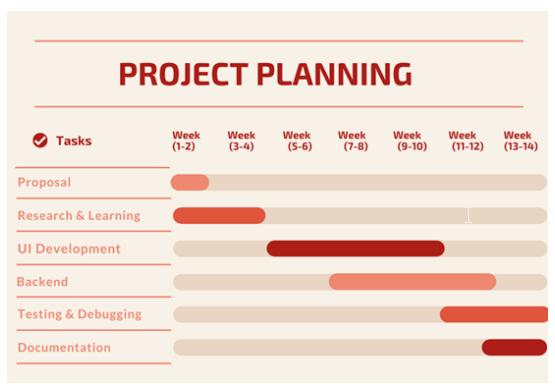
\includegraphics[width=0.8\textwidth]{gantt.png}
  \caption{Project timeline and task distribution}
  \label{fig:gantt}
\end{figure}

\chapter{Implementation and Results}
\section{System Modules and Core Functionality}
The implemented banking system is organized into several functional modules that work together to support the complete transaction lifecycle. The authentication module handles user registration and login, the account module manages balance-related operations, the transfer module creates pending transactions, and the admin module reviews and approves or rejects those requests. These modules communicate through a shared SQLite-backed data layer, which ensures that account updates remain consistent and traceable.

\section{User Workflow and Transaction Processing}
A typical user session begins with registration and login, followed by account access and balance viewing. Once a user submits a transfer request, the system records the transaction as pending and stores the required sender, receiver, amount, and note information in the database. The administrator can then review pending transactions and decide whether to approve or reject them. If approved, the system updates both account balances in a controlled manner so that the transaction is reflected consistently in the records.

\begin{figure}[H]
  \centering
  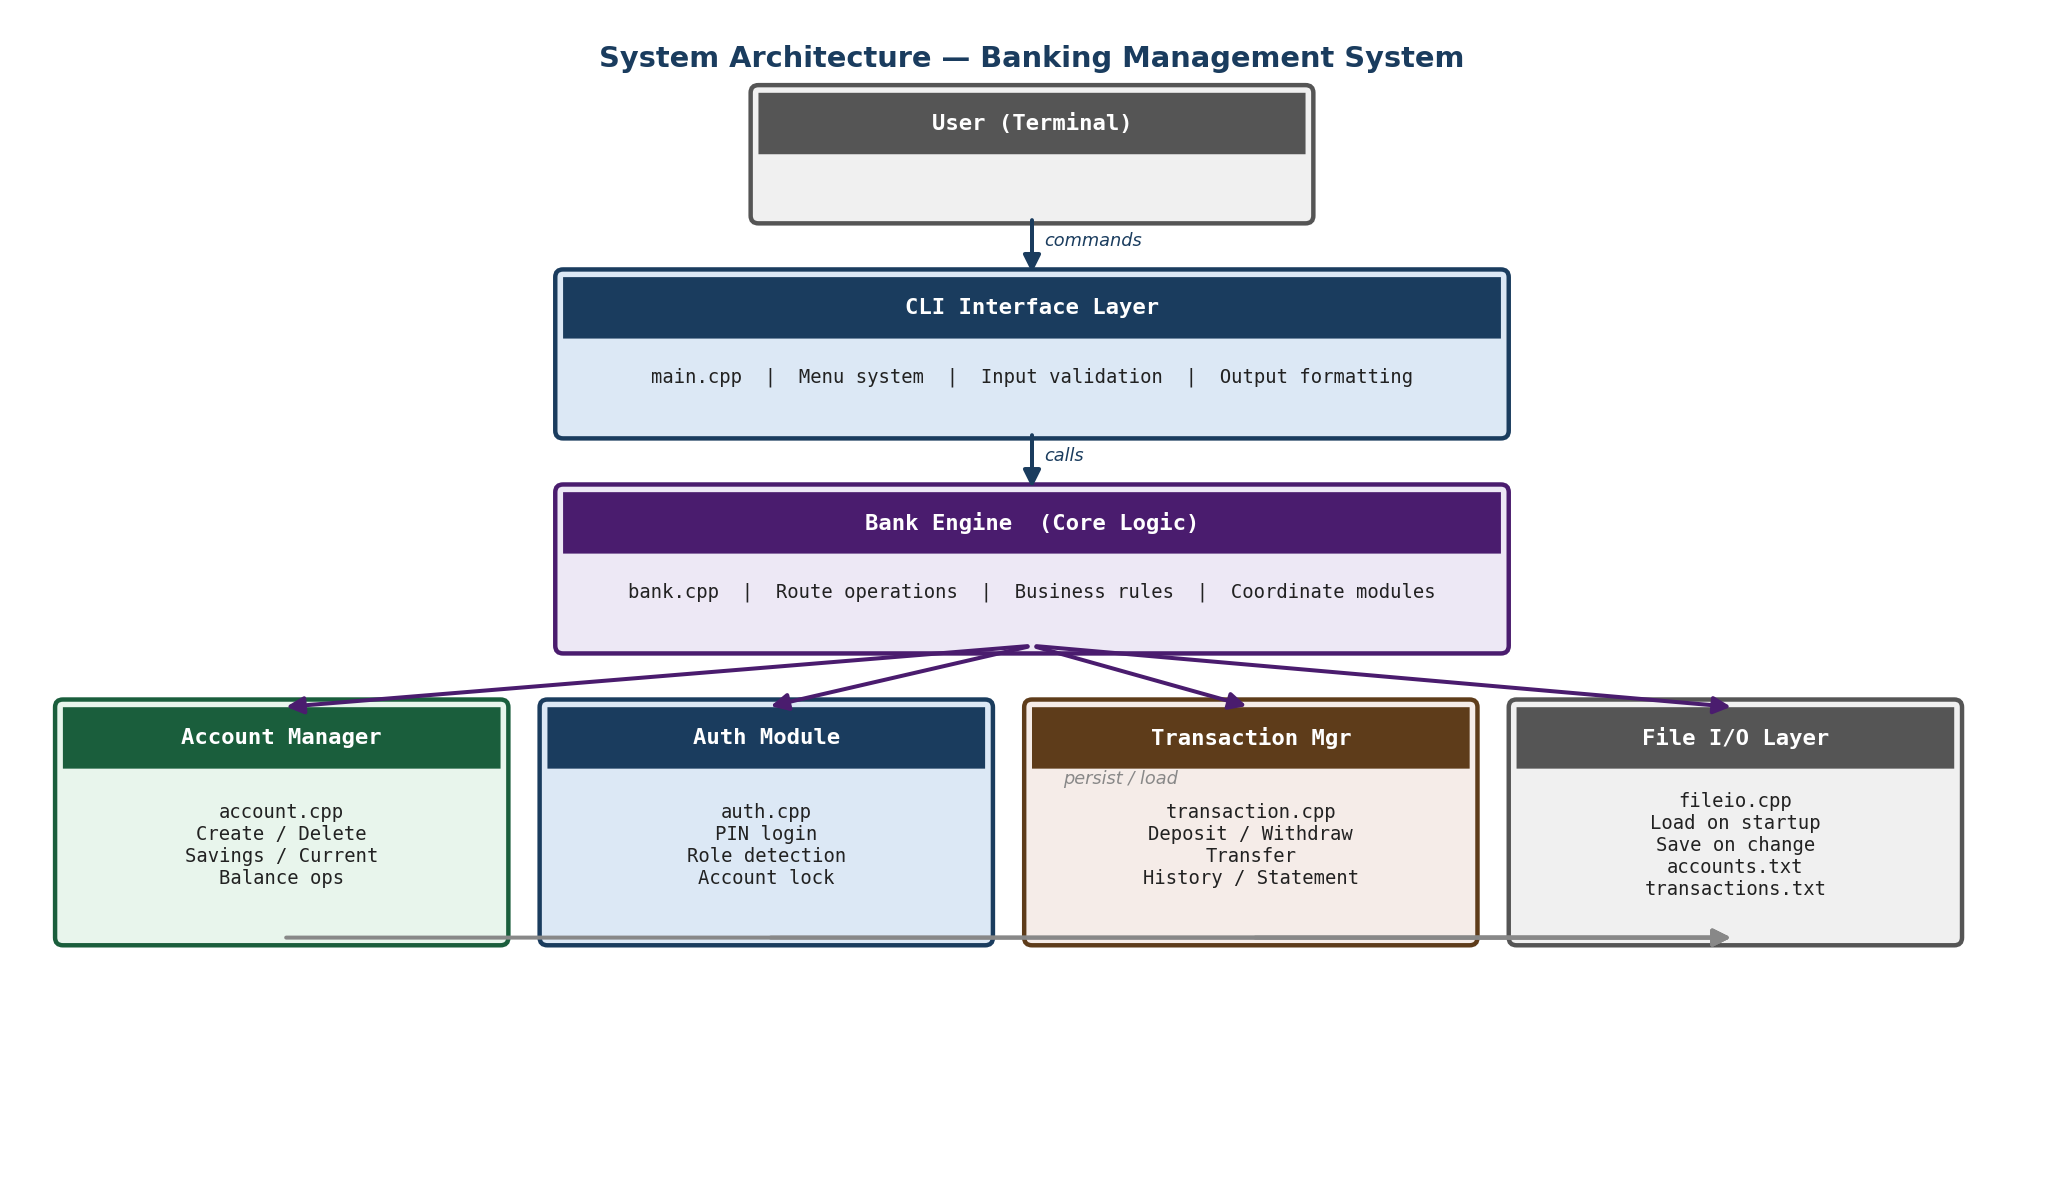
\includegraphics[width=0.72\textwidth]{image2.png}
  \caption{System architecture of the Banking Management System}
  \label{fig:architecture}
\end{figure}

\begin{figure}[H]
  \centering
  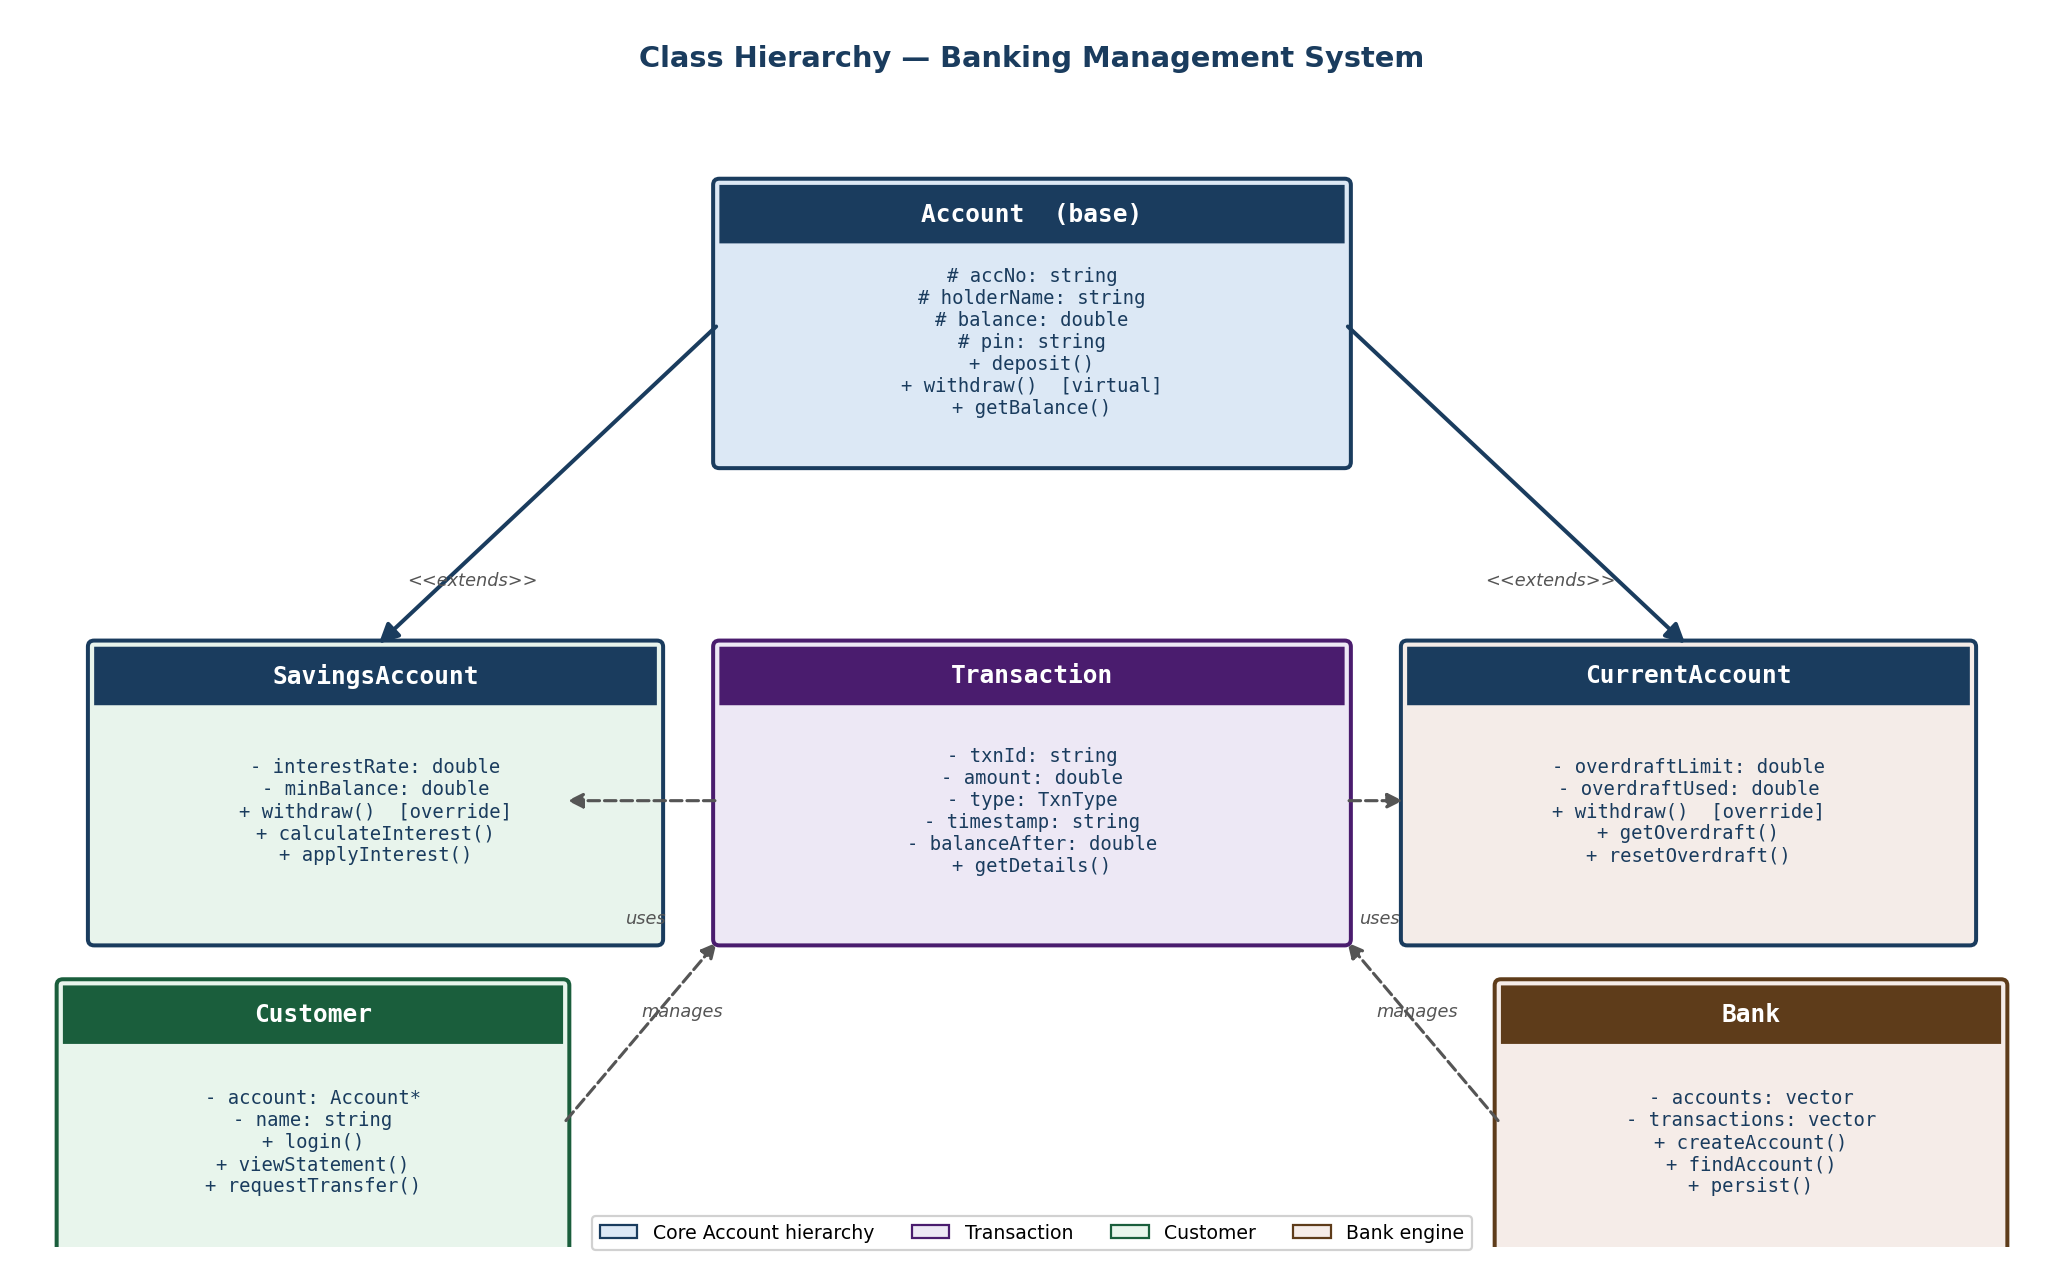
\includegraphics[width=0.72\textwidth]{image3.png}
  \caption{Class hierarchy for the core banking components}
  \label{fig:classhierarchy}
\end{figure}

\section{Admin Interface and Approval Flow}
The administrator interface provides an efficient way to manage pending transfers and monitor account activity. From the admin panel, the supervisor can inspect transaction requests, verify the involved accounts, and decide whether to approve or reject each transaction. This design closely reflects the approval-based control often used in simple financial systems and helps enforce a review step before funds are moved.

\begin{figure}[H]
  \centering
  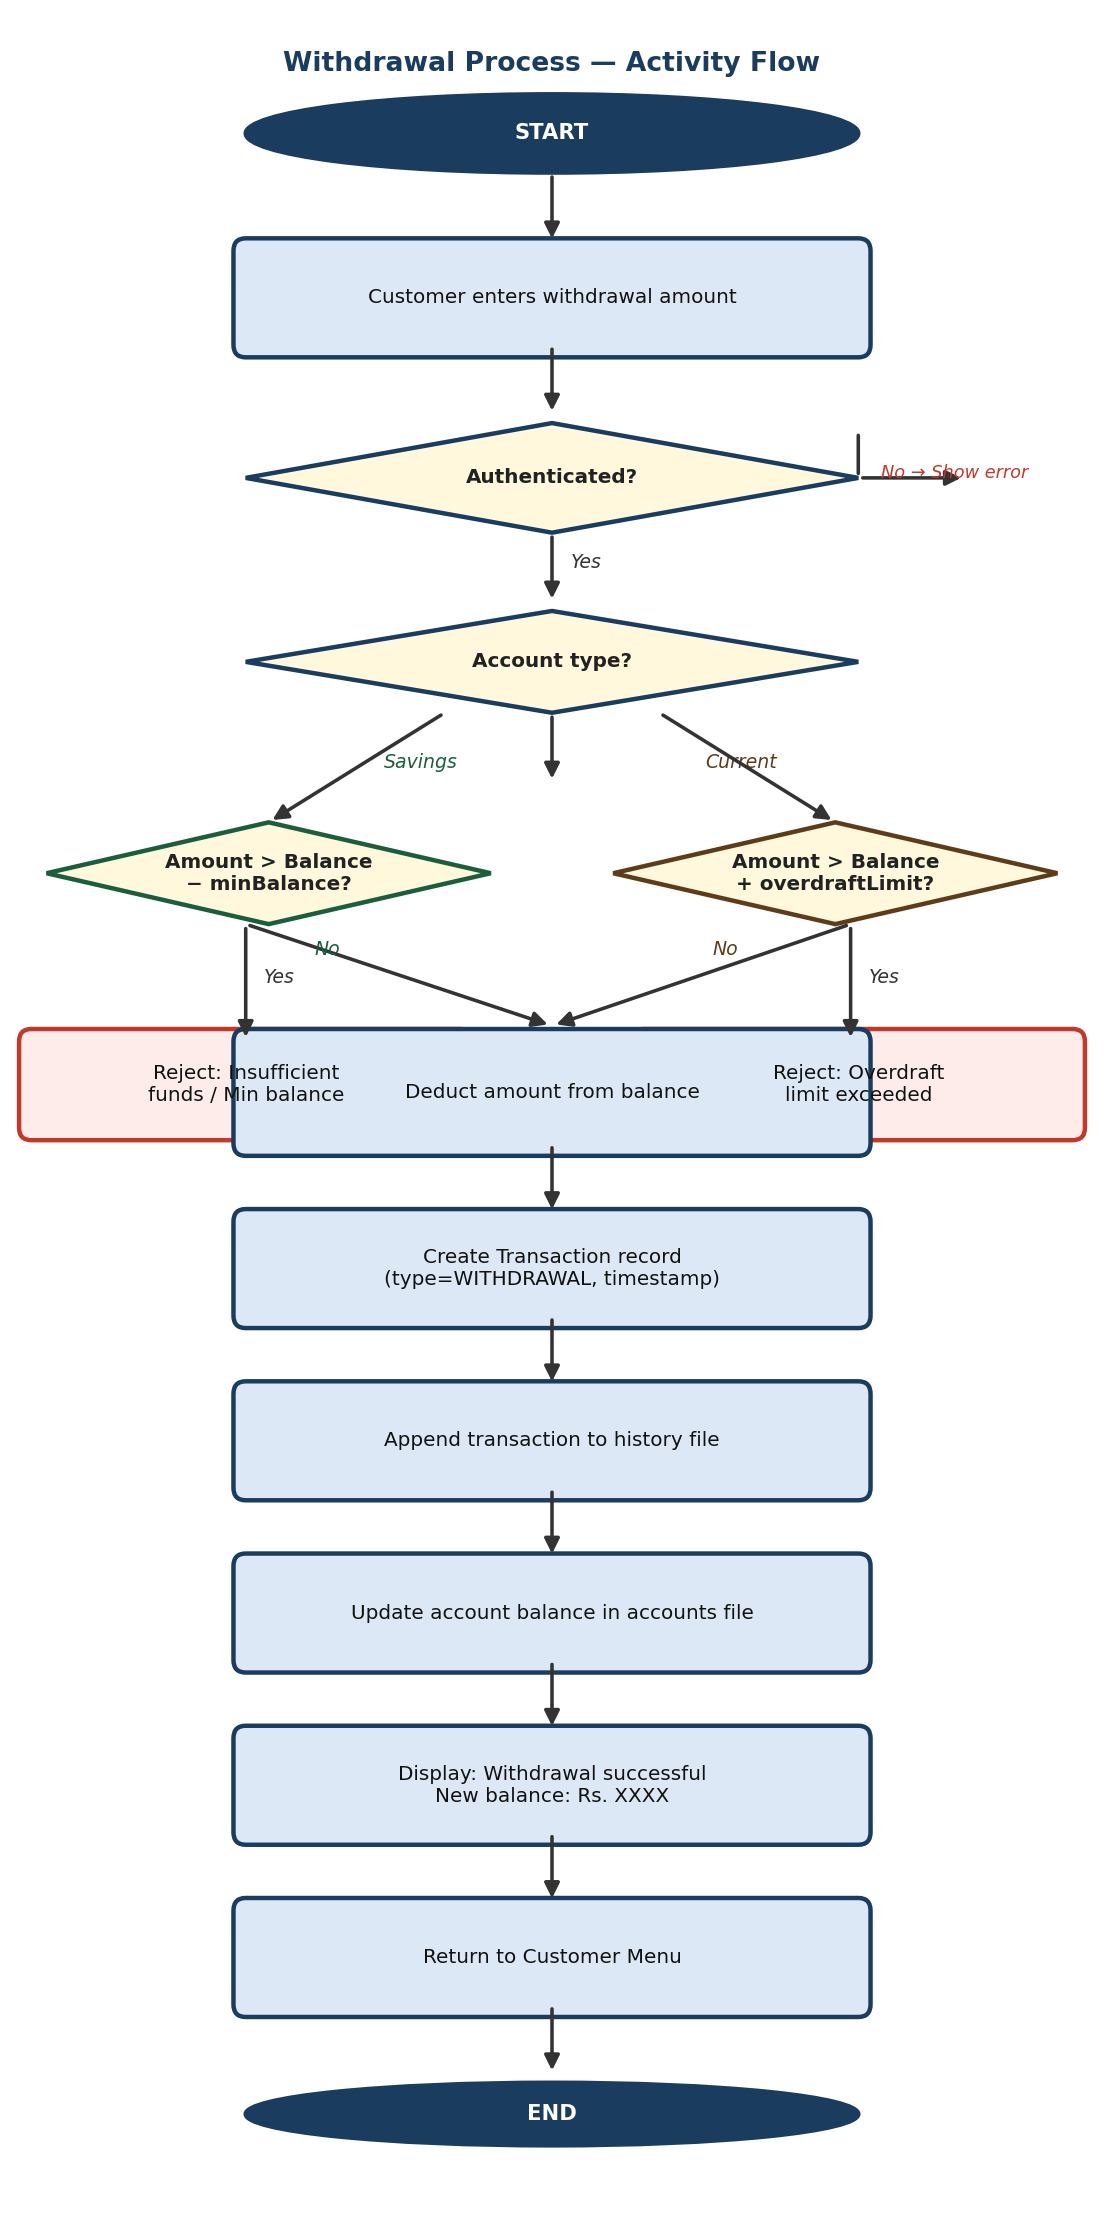
\includegraphics[width=0.72\textwidth]{image4.png}
  \caption{Withdrawal process activity flow used as an example of transaction handling}
  \label{fig:transactionflow}
\end{figure}

\section{Testing and Observations}
The system was tested through a sample execution flow that covered registration, login, balance viewing, transfer submission, and admin approval. The test run confirmed that the application could successfully create accounts, store transactions, and update balances after approval. The captured transcript in the appendix provides additional evidence of the working flow and the behavior of the console interface during execution.

\section{Feature Summary}
The core features implemented in this system include:
\begin{itemize}
  \item secure user registration and authentication,
  \item customer account balance tracking,
  \item pending transfer request creation,
  \item administrator approval and rejection workflows,
  \item persistent SQLite-backed data storage for users, accounts, and transaction history.
\end{itemize}

\begin{table}[H]
  \centering
  \caption{Summary of core system features}
  \begin{tabular}{|p{0.45\textwidth}|p{0.45\textwidth}|}
    \hline
    \textbf{Feature} & \textbf{Status} \\
    \hline
    User registration and login & Implemented \\
    \hline
    Account balance management & Implemented \\
    \hline
    Pending transfer workflow & Implemented \\
    \hline
    Admin approval and review & Implemented \\
    \hline
    Persistent database storage & Implemented \\
    \hline
  \end{tabular}
\end{table}

\chapter{Conclusion and Future Work}
The Banking Management System developed in this project successfully demonstrates the core concepts of banking software through a compact, database-backed console application. The project provides a solid foundation for further enhancement, including a graphical user interface, stronger authentication practices, more detailed reporting, and support for additional banking features such as loan management or statement generation.

\cleardoublepage
\addcontentsline{toc}{chapter}{References}
\bibliographystyle{apalike}
\bibliography{report}

\cleardoublepage
\chapter*{Appendix A: Console Output and Run Transcript}
\addcontentsline{toc}{chapter}{Appendix A: Console Output and Run Transcript}
The sample console transcript captured during project testing is included below and is also stored in the figures folder for reference.
\verbatiminput{figures/console_output.txt}

\end{document}




